
%%%%%%%%%%%%%%%%%%%%%%%%%%%%%%%%%%%%%%%%%%%%%%%%%%%%%%%%%%%%%%%%%%%%%%%%%%%%%%%%%%%%%%%
% Denna fil kompileras (pdflatex designspec.tex)
% Inga ändringar bör behöva göras
% Saknar din installation bibliotek? Installera dem eller skrik på dokumentansvarig.
%%%%%%%%%%%%%%%%%%%%%%%%%%%%%%%%%%%%%%%%%%%%%%%%%%%%%%%%%%%%%%%%%%%%%%%%%%%%%%%%%%%%%%%

% Document props and library inclusions
\documentclass[10pt,a4paper]{report} 
\usepackage[utf8]{inputenc} 
\usepackage[english]{babel}
\usepackage{mathtools,tikz,textcomp,fixltx2e,color,fullpage,graphicx,afterpage,float,parskip,xfrac,gensymb,titlesec,etoolbox,pdfpages,hyperref}
\usetikzlibrary{calc,matrix,positioning,arrows,shapes,trees,plotmarks,decorations.markings}
\usepackage[font={small,it}]{caption}
\usepackage[europeancurrents,europeanvoltages,europeanresistors,europeaninductors,smartlabels]{circuitikz}
\usepackage[font={small,it}]{caption} %% Italics in captions

\setcounter{secnumdepth}{2} % Levels enumerated
\setcounter{tocdepth}{3} % ToC levels enumerated

% PDF props
\hypersetup{
  bookmarks=true,              % show bookmarks bar?
  bookmarkstype=toc,
  bookmarksopenlevel=\maxdimen
  unicode=true,                % non-Latin characters in Acrobat’s bookmarks
  pdftoolbar=true,             % show Acrobat’s toolbar?
  pdfmenubar=true,             % show Acrobat’s menu?
  pdffitwindow=false,          % window fit to page when opened
  pdfstartview={FitH},         % fits the width of the page to the window
  pdftitle={Design Specification},         % title
  pdfauthor={Petersson, Oscar}, % author
  pdfsubject={TSIU03},          % subject of the document
  pdfkeywords={TSIU03}          % list of keywords
  pdfnewwindow=true,           % links in new window
  hidelinks,                   % hide links (removing color and border)
  linktocpage=true,
  linktoc=all,                 % parts of TOC made into links
  pdfdisplaydoctitle=true      %display document title instead of file name in title bar
}
\urlstyle{same}

\graphicspath{{./fig/}} % including pictures from here

%% First Page Information
\author{Niklas Blomqvist, Philip Johansson, Matteus Laurent, Johan Levinsson, Oscar Petersson, Erik Peyronson}
\title{Group 41 - Design Specification}
\date{\today}
\newcommand{\course}{System Design - Project, HT15}
\newcommand{\coursenumber}{TSIU03, Linköpings universitet}
\newcommand{\programme}{Högskoleingenjörsutbildning i datateknik, 180 hp}
\newcommand{\examiner}{Petter Källström}
\newcommand{\institution}{Department of Electrical Engineering (ISY)}
\newcommand{\reptype}{Design Specification}

%\newcommand{\includelogo}{\includegraphics[width=48 mm]{LiTH_sigill_sv.pdf}\makeatletter\begin{center}\vskip 4.5cm}
\newcommand{\excludelogo}{\makeatletter\begin{center}~\vfill}

%% Proper Chapter Head
\makeatletter
\renewcommand{\@makechapterhead}[1]{%
  \vspace*{50 pt}%
          {\setlength{\parindent}{0pt} \raggedright \normalfont
            \bfseries\Huge
            \ifnum \value{secnumdepth}>1
            \if@mainmatter\thechapter.\ \fi%
            \fi
            #1\par\nobreak\vspace{40 pt}}}
\makeatother

\begin{document}

\pagestyle{empty}
%\includelogo
 \excludelogo
  \Large{\@author}\vskip .3cm
  \textbf{\LARGE{\@title}}\vskip .2cm
  \large{\programme}
  \vfill
\end{center}
\reptype{} - \@date\hfill Supervisor:\\
\textbf{\course}\hfill\examiner\\
\coursenumber\hfill\institution
\makeatother
\newpage
\afterpage{\null\newpage}
\thispagestyle{empty}

%% Table of Contents
\addtocontents{toc}{\protect\hypertarget{toc}{}}
\tableofcontents\label{sec:toc}
\addtocontents{toc}{\protect\thispagestyle{empty}}
\cleardoublepage

Project 41 is based around audio signal processing. The audio input and output both go through the WM8731 chip on a DE2 board. Meanwhile, the hardware settings are controlled from a PS/2 keyboard and displayed on a VGA screen. The hardware settings to be implemented are a volume control and a balance control. In addition, an interface consisting of the input and output power level along with appropriate indicators as stated in the requirement specification.

The WM8731 is a stereo codec, which in Project 41 is used as a bridge between the audio source and a class-D amplifier. The custom hardware controls the WM8731 as the analysis of the input controls and encoding the graphical output. The output sound sent to a Class-D amplifier is then allowed further amplification through another instance of pulse width modulation within the amplifier.


\input{tex/manual.tex}
\begin{frame}
  \frametitle{Overview}
    \begin{figure}
      \centering
      \includegraphics[scale=.23]{overview}
    \end{figure}


    \begin{itemize}
      \item Keyboard
      \item Vol\_Bal
      \item Snd\_Driver
      \item Analysis
      \item VGA\_Driver
    \end{itemize}

\end{frame}

\begin{frame}
  \frametitle{Keyboard Decoding}
  \framesubtitle{Scan Code Detection}
  \begin{itemize}
  \item<1->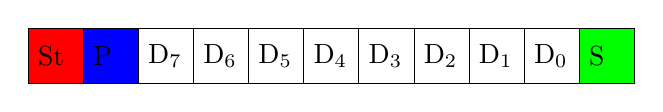
\begin{tikzpicture}[y=.7 cm, x=.7 cm]
    \draw(0,0) rectangle (11,1);
    \draw[fill=green] (10,0) rectangle (11,1);
    \draw[fill=blue] (1,0) rectangle (2,1);
    \draw[fill=red] (0,0) rectangle (1,1);
    \foreach \x in {1,...,10}
    \draw (\x, 0 ) -- ( \x, 1 );
    \draw (10,.5) node[anchor=west]{S};
    \draw (9,.5) node[anchor=west]{D$_0$};
    \draw (8,.5) node[anchor=west]{D$_1$};
    \draw (7,.5) node[anchor=west]{D$_2$};
    \draw (6,.5) node[anchor=west]{D$_3$};
    \draw (5,.5) node[anchor=west]{D$_4$};
    \draw (4,.5) node[anchor=west]{D$_5$};
    \draw (3,.5) node[anchor=west]{D$_6$};
    \draw (2,.5) node[anchor=west]{D$_7$};
    \draw (1,.5) node[anchor=west]{P};
    \draw (0,.5) node[anchor=west]{St};
  \end{tikzpicture}
  
  \item<2-2>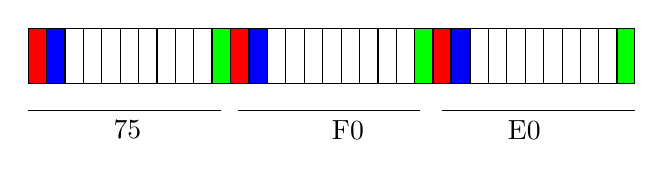
\begin{tikzpicture}[x=.7 cm, y=.7 cm]
    \draw(0,-2) rectangle (11,-1);
    \foreach \x in {3.333,7,10.666}
    \draw[fill=green] (\x,-2) rectangle (\x+.334,-1);
    \foreach \x in {.333,4,7.666}
    \draw[fill=blue] (\x,-2) rectangle (\x+.334,-1);
    \foreach \x in {0,3.666,7.333}
    \draw[fill=red] (\x,-2) rectangle (\x+.334,-1);
    \foreach \x in {0,.333,.667,...,11}
    \draw (\x, -2 ) -- ( \x, -1 );

    \draw (0,-2.5) -- (3.5,-2.5);
    \draw (1.8,-2.5) node[anchor=north]{75};
    \draw (3.8,-2.5) -- (7.1,-2.5);
    \draw (5.8,-2.5) node[anchor=north]{F0};
    \draw (7.5,-2.5) -- (11,-2.5);
    \draw (9,-2.5) node[anchor=north]{E0};
  
  \end{tikzpicture}
    
  \item<3->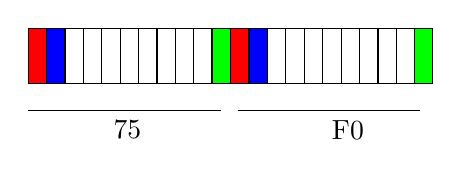
\begin{tikzpicture}[x=.7 cm, y=.7 cm]
    \draw(0,-2) rectangle (7.333,-1);

    \foreach \x in {3.333,7}
    \draw[fill=green] (\x,-2) rectangle (\x+.334,-1);
    \foreach \x in {.333,4}
    \draw[fill=blue] (\x,-2) rectangle (\x+.334,-1);
    \foreach \x in {0,3.666}
    \draw[fill=red] (\x,-2) rectangle (\x+.334,-1);
    \foreach \x in {0,.333,.667,...,7.333}
    \draw (\x, -2 ) -- ( \x, -1 );

    \draw (0,-2.5) -- (3.5,-2.5);
    \draw (1.8,-2.5) node[anchor=north]{75};
    \draw (3.8,-2.5) -- (7.1,-2.5);
    \draw (5.8,-2.5) node[anchor=north]{F0};
  
  \end{tikzpicture}
  \end{itemize}
  
\end{frame}

\subsection{Vol\_Bal:current\_vol\_bal}

The Volume/Balance module (\verb=Vol_Bal=) acts as the hub for processing incoming digital audio signals, forwarded from WM8731 via the SndDriver module. As such, \verb=Vol_Bal= also keeps internal registers that holds current volume and balance levels as signed 4-bit values (legal values range from -5 to 5 where 0 represents no adjustment). These registers update via the one-hot coded input signal \verb=kb_input= applied by the \verb=Keyboard= module, and the values they hold are used as signals (\verb=i_volume_lvl=, \verb=i_balance_lvl=) for the internal modules that process the \verb=LADC= and \verb=RADC= inputs. Furthermore, the signals are also directed as outputs connected to the VGADriver module so that they can be rendered on the screen.

The main function of the Volume/Balance module is to make requested adjustments to incoming values \verb=LADC= and \verb=RADC=, which represent a measured amplitude respectively at a certain time. They will first be adjusted for volume by a function $A_{new} = A_{old} * \sqrt{2}^n$ where $A$ is the amplitude and $n$ is the signed value in the volume level register. The new values are forwarded for balance adjustment jointly with a ready signal to inform that the \verb=adj_LADC= (or \verb=RADC=) should be read. Same processing is applied in the \verb=Bal_Adj= module to produce the \verb=LDAC= and \verb=RDAC= outputs conveyed to SndDriver and Analysis.

As a result, the user can digitally adjust volume -15/+15 dB and also decrease volume by another 15 dB on a single left/right audio channel.

(Lastly, this design will be simplified by combining volume and balance adjustment volumes)

The \verb=Analysis= module has one responsibility. It reads the ADC signal and puts out information on how to draw two bars (one for each speaker) that represent the amplitude of said signal. Since we want bars for before and after modulation, we'll use two instances of the same module. 

The required inputs include a left or right selection signal to specify which stereo channel we're about to analyse, two ADC signals (left and right), a clock signal that's synced with the \verb=VGA_driver= since the polling rate of the \verb=Snd_Driver= and \verb=Vga_Driver= differ.  

There are two output signals (once again, one left, one right). They determine the height of the bar which the \verb=VGA_Driver= should render. 

\verb=lrsel= determines which stereo channel should be read and thus which bar height should be written to at any given time.

%Frame 1 Kort introduktion

\begin{frame}
  \frametitle{VGA\_driver}
  \framesubtitle{Overview}
  \begin{itemize}
  \item<1-> Based on Laboration 2.
  \item<2-> Two new submodules.
    \begin{itemize}
    \item<3-> bar\_tender.
    \item<4-> bar\_mixer.
    \end{itemize}
  \item<5-> Nånting bra testest.
  \end{itemize}
\end{frame}

%Frame 2 Överiktsbild

\begin{frame}
  \frametitle{VGA\_driver}
  \framesubtitle{System overview}
  \begin{figure}[H]
    \centering 
    \includegraphics[scale=0.80]{picture_xy.png} 
    %\caption{Entity-Relationship diagram} 
    \label{fig:picture_xy.png}
  \end{figure}
\end{frame}

\begin{frame}
  %\begin{itemize}
  %\item<1-> test
  %\item<2-> test2
  %\end{itemize}
  
  \frametitle{VGA\_driver}
  \framesubtitle{System overview}
  \begin{figure}[l]
    \centering 
    \includegraphics[scale=0.40]{bar_mixer.png} 
    %\caption{Entity-Relationship diagram} 
    \label{fig:bar_mixer.png}
  \end{figure}
\end{frame}

\input{tex/demo.tex}


\end{document}
